\chapter{Water adsorption in silica}

\vspace{-1cm} \noindent \textcolor{graytitle}{\textit{{\Large Dealing with a varying number of molecules}}\vspace{0.5cm} }

\noindent \hspace{-0.45cm}\begin{wrapfigure}{r}{4cm}
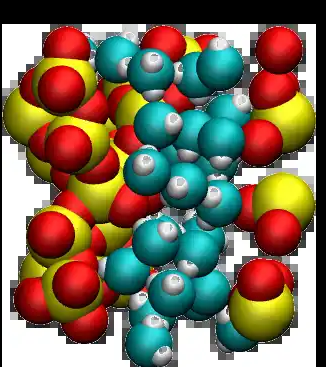
\includegraphics[width=4cm]{tutorials/level3/water-adsorption-in-silica/avatar-light.png}
\end{wrapfigure}

\noindent The objective of this tutorial is to combine molecular
dynamics and grand canonical Monte Carlo simulations to
compute the adsorption of water molecules in a cracked silica material.
This tutorial illustrates the use of the grand canonical
ensemble in molecular simulation, an open ensemble in which the number of 
molecules or atoms is not constant.

\section{Generation of the silica block}

\noindent Let us first generate a block of amorphous silica (SiO2). To do
so, we are going to replicate a building block containing 3
Si and 6 O atoms. 

Create two folders side by side, and name them respectively \textit{Potential/}
and \textit{SilicaBlock/}.
An initial data file for the SiO atoms can be
downloaded by clicking \href{../../../../../inputs/level3/water-adsorption-in-silica/SilicaBlock/SiO.data}{here}.
Save it in \textit{SilicaBlock/}. This data file
contains the coordinates of the 9 atoms, their masses, and
their charges. The fine can be directly read by LAMMPS using the
\textit{read$\_$file} command. Let us replicate these atoms using
LAMMPS, and apply an annealing procedure to obtain a block
of amorphous silica.

\begin{tcolorbox}[colback=mylightblue!5!white,colframe=mylightblue!75!black,title=About annealing procedure]
The annealing procedure consists of adjusting the system temperature in successive steps.
Here, a large initial temperature is chosen to ensure the melting of the SiO2 structure.
Then, several steps are used to progressively cool down the system until it solidifies and forms 
amorphous silica. Depending on the material, different cooling velocities can sometimes
lead to different crystal structure or different degree of defect.
\end{tcolorbox}

\noindent \subsection{Vashishta potential}

Create a new input file named \textit{input.lammps} in the \textit{SilicaBlock/} folder, and copy
the following lines in it:

\begin{lcverbatim}
units metal
boundary p p p
atom_style full
pair_style vashishta
neighbor 1.0 bin
neigh_modify delay 1
\end{lcverbatim}

\noindent The main difference between the previous tutorials is the use of 
the Vashishta pair style. Download the Vashishta potential by
clicking \href{../../../../../inputs/level3/water-adsorption-in-silica/Potential/SiO.1990.vashishta}{here}, and copy it within the \textit{Potential/} folder.

\begin{tcolorbox}[colback=mylightblue!5!white,colframe=mylightblue!75!black,title=About the Vashishta potential]
The \href{https://pubmed.ncbi.nlm.nih.gov/9993674/}{Vashishta}
potential is a bond-angle energy based potential, it
deduces the bonds between atoms from their relative
positions. Therefore, there is no need to provide bond
and angle information as we do with classic force fields
like GROMOS or AMBER.

Note that Vashishta potential requires the use of metal units system. 

Bond-angle energy based potentials
are more computationally heavy than classical force
fields and require the use of a smaller timestep, but
they allow for the modelling of bond formation and
breaking, which is what we need here as we want to create
a crack in the silica.
\end{tcolorbox}

\noindent Let us then import the system made of 9 atoms, replicate it four times in all three
directions of space, thus creating a system with 576 atoms.

\begin{lcverbatim}
read_data SiO.data
replicate 4 4 4
\end{lcverbatim}

\noindent Then, let us specify the pair coefficients by indicating
that the first atom type is Si, and the second is O. Let us also
add a dump command for printing out the positions of the
atoms every 5000 steps:

\begin{lcverbatim}
pair_coeff * * ../Potential/SiO.1990.vashishta Si O
\end{lcverbatim}

\noindent Let us add some commands to help us follow the evolution of the system,
such as its temperature, volume, and potential-energy:

\begin{lcverbatim}
dump dmp all atom 5000 dump.lammpstrj
variable myvol equal vol
variable mylx equal lx
variable myly equal ly
variable mylz equal lz
variable mypot equal pe
fix myat1 all ave/time 10 100 1000 v_mytemp file temperature.dat
fix myat2 all ave/time 10 100 1000 v_myvol v_mylx v_myly v_mylz file dimensions.dat
fix myat3 all ave/time 10 100 1000 v_mypot file potential-energy.dat
thermo 1000
\end{lcverbatim}

\noindent \subsection{Annealing procedure}

Finally, let us create the last part of our script. The
annealing procedure is the following: we first start with a
small phase at 6000 K, then cool down the system to 4000 K
using a pressure of 100 atm. Then we cool down the system
further while also reducing the pressure, then perform a
small equilibration step at the final desired condition, 300
K and 1 atm.
\textit{Disclaimer --} I created this procedure by intuition and
not from proper calibration, do not copy it without
making your own tests if you intend to publish your
results.

\begin{lcverbatim}
velocity all create 6000 4928459 rot yes dist gaussian
fix npt1 all npt temp 6000 6000 0.1 iso 100 100 1
timestep 0.001
run 50000
fix npt1 all npt temp 6000 4000 0.1 aniso 100 100 1
run 50000
fix npt1 all npt temp 4000 300 0.1 aniso 100 1 1
run 200000
fix npt1 all npt temp 300 300 0.1 aniso 1 1 1
run 50000
write_data amorphousSiO.data
\end{lcverbatim}

\noindent \begin{tcolorbox}[colback=mylightblue!5!white,colframe=mylightblue!75!black,title=Anisotropic versus isotropic barostat]
Here, an isotropic barostat is used for the melted phase at 6000 K, and then 
an anisotropic barostat when cooling down the system. With the anisotropic 
barostat, all three directions of space are adjusted independently from one another. Such
anisotropic barostat is usually a better choice for a solid phase, 
when there is no reason for the final solid phase to
have the same dimensions along all 3 axis. For a
liquid or a gas, the isotropic barostat is usually the best choice.
\end{tcolorbox}

\noindent The simulation takes about 15-20 minutes on 4 cpu cores.
Let us check the evolution of the temperature from the \textit{temperature.dat} file.
Apart from an initial spike (may be due to an initial bad configuration, probably harmless here),
the temperature follows well the desired annealing procedure:

\begin{figure}
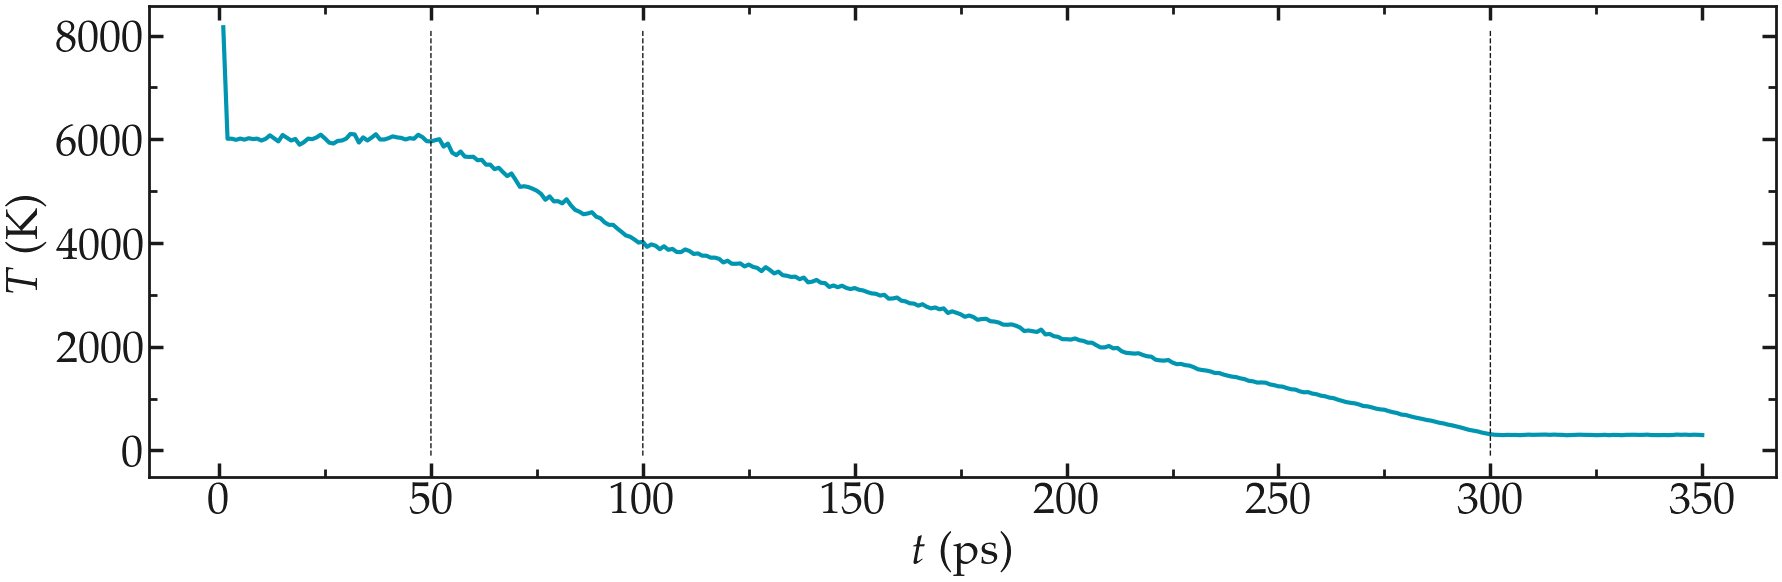
\includegraphics[width=\linewidth]{tutorials/level3/water-adsorption-in-silica/temperature_evolution-light.png}
\end{figure}

Let us also make sure that the box was indeed deformed isotropically during the first 
stage of the simulation, and then anisotropically by plotting lx (blue), ly (orange), and lz:

\begin{figure}
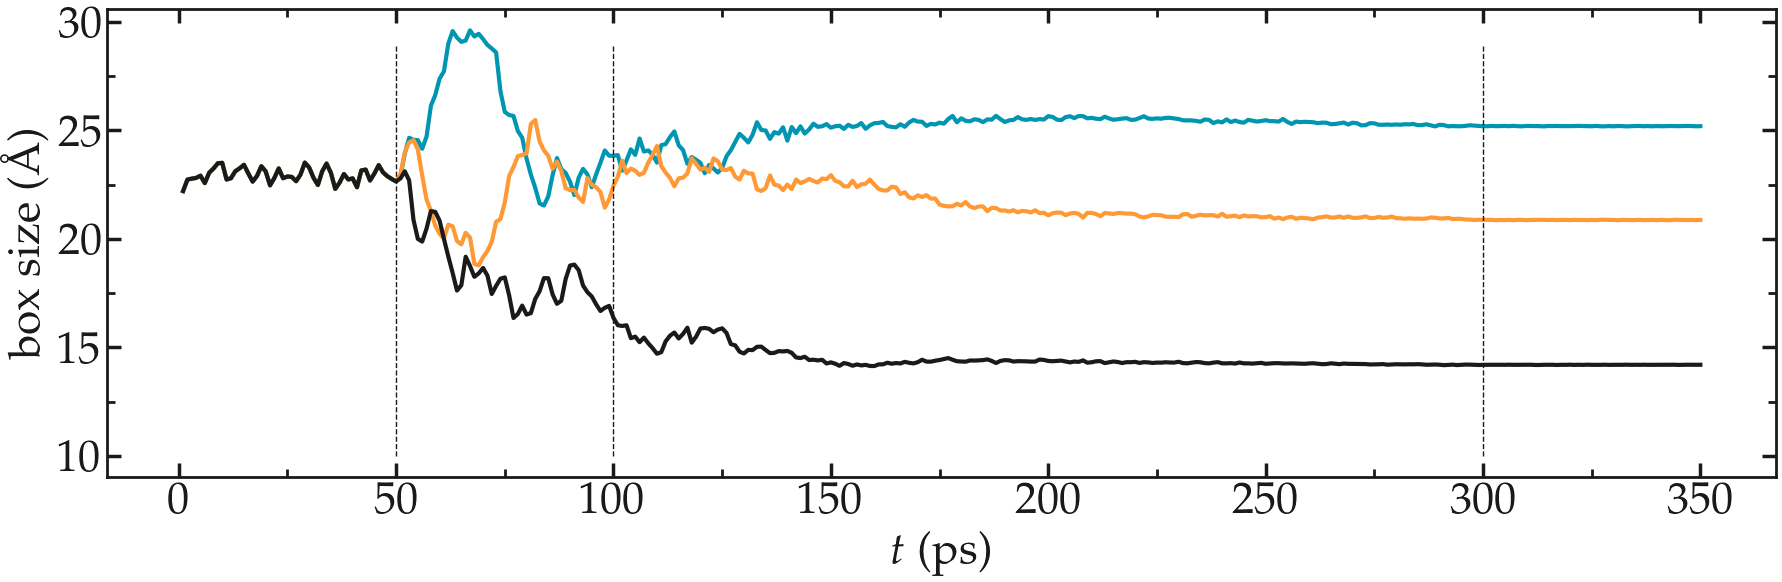
\includegraphics[width=\linewidth]{tutorials/level3/water-adsorption-in-silica/dimensions_evolution-light.png}
\end{figure}

\hspace{-0.45cm}\begin{wrapfigure}{r}{4cm}
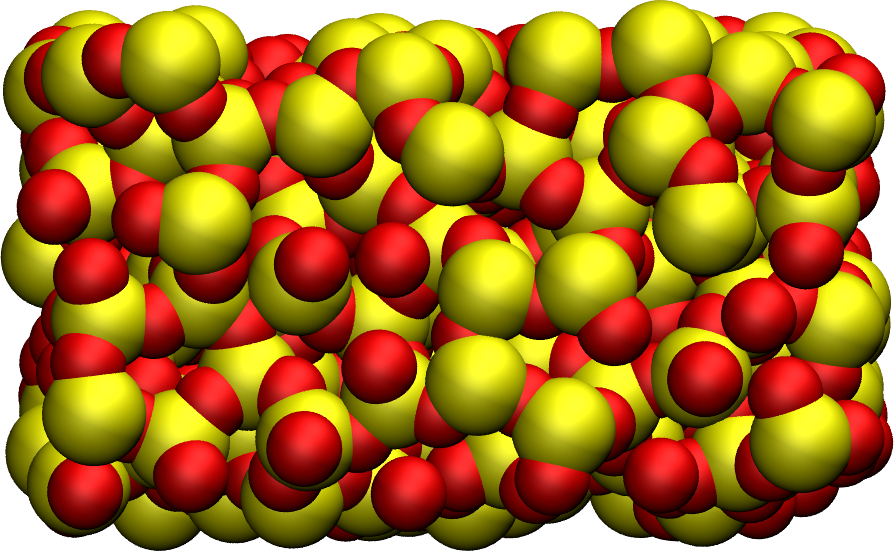
\includegraphics[width=4cm]{tutorials/level3/water-adsorption-in-silica/generated-silica-light.png}
\end{wrapfigure}

\noindent The snapshot on the side shows the final amorphous silica (SiO2).
After running the simulation, the final LAMMPS topology file named
\textit{amorphousSiO.data} will be located in \textit{SilicaBlock/}. Alternatively, if you are only interested in the
next steps of this tutorial, you can download it by clicking
\href{../../../../../inputs/level3/water-adsorption-in-silica/SilicaBlock/amorphousSiO.data}{here}.

\begin{tcolorbox}[colback=mylightblue!5!white,colframe=mylightblue!75!black,title=Tip for research project]
In the case of a research project, the validity of the generated
structure must be tested and compared to reference values, ideally from
experiments. 

For instance, radial distribution functions or Young modulus
can both be compared to experimental values. This is beyond the
scope of this tutorial.
\end{tcolorbox}

\noindent \section{Cracking the silica}

Let us dilate the block of silica to create a
crack. Create a new folder called \textit{Cracking/} next to \textit{SilicaBlock/}, and create a
new input.lammps file starting with:

\begin{lcverbatim}
units metal
boundary p p p
atom_style full
neighbor 1.0 bin
neigh_modify delay 1
read_data ../SilicaBlock/amorphousSiO.data
pair_style vashishta
pair_coeff * * ../Potential/SiO.1990.vashishta Si O
dump dmp all atom 1000 dump.lammpstrj
\end{lcverbatim}

\noindent Then, let us progressively increase the size of the
box in the z direction, thus forcing the silica to deform and crack. To do
so, we are going to make a loop using the jump command. At
every step of the loop, the box dimension over x will
be multiplied by a factor 1.005. Here, we use a NVT
thermostat because we want to impose a deformation of the
volume.

\begin{tcolorbox}[colback=mylightblue!5!white,colframe=mylightblue!75!black,title=NVT vs 2D barostat]
Here, box deformations are applied in the x-direction, while the 
y and z box dimensions are kept constants. 
Another possible choice would be to apply a barostat along the y and z 
direction, allowing the system more freedom to deform. In LAMMPS, this 
can be done by using :
\begin{lcverbatim}
fix npt1 all npt temp 300 300 0.1 y 1 1 1 z 1 1 1
\end{lcverbatim}

\noindent instead of:

\begin{lcverbatim}
fix nvt1 all nvt temp 300 300 0.1
\end{lcverbatim}

\noindent Here, the latter command will be used (see below), but feel free to improvise.
\end{tcolorbox}

\noindent Add the following lines to the input script:

\begin{lcverbatim}
fix nvt1 all nvt temp 300 300 0.1
timestep 0.001
thermo 1000
variable var loop 45
label loop
change_box all x scale 1.005 remap
run 2000
next var
jump input.lammps loop
run 20000
write_data dilatedSiO.data
\end{lcverbatim}

\noindent Use different factor (1.005) or different number of 
loop (45) if you want to generate different defects in the silica.

\hspace{-0.45cm}\begin{wrapfigure}{r}{4cm}
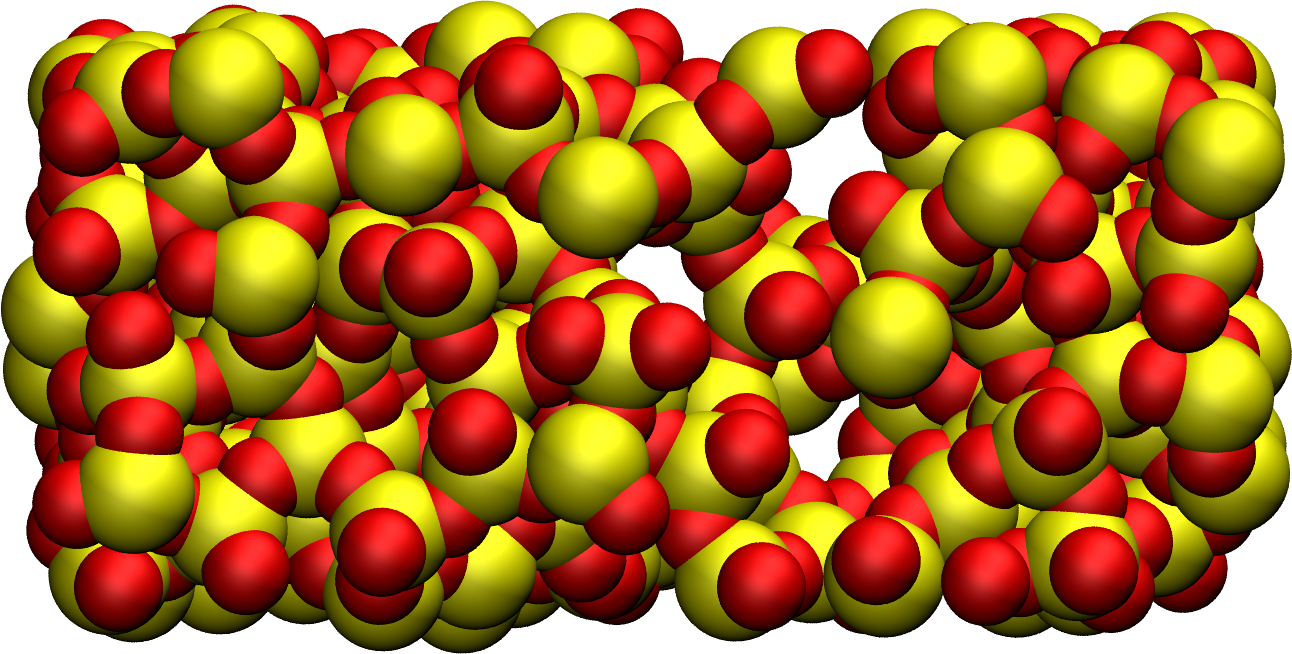
\includegraphics[width=4cm]{tutorials/level3/water-adsorption-in-silica/cracked-light.png}
\end{wrapfigure}

\noindent The snapshot on the side shows the block of silica with holes and deformed bonds.
After the dilatation, a final equilibration step of 20
picoseconds is performed. If you look at the dump file
produced after executing this script, or at \href{https://www.youtube.com/watch?v=8rBqYIcTgno&ab_channel=SimonGravelle}{this video},
you can see the dilatation occurring step-by-step, and the
atoms adjusting progressively to the box size. 

At first, the deformations
are reversible (elastic regime). At some point, bonds
start breaking and dislocations appear (plastic regime). 

Alternatively, you
can download the final state directly by clicking
\href{../../../../../inputs/level3/water-adsorption-in-silica/Cracking/dilatedSiO.data}{here}. The final system, with the crack, resembles:

\begin{tcolorbox}[colback=mylightblue!5!white,colframe=mylightblue!75!black,title=Passivated silica]
In ambient conditions, Some of the surface SiO2 atoms are chemically
passivated by forming covalent bonds with hydrogen (H)
atoms. For the sake of simplicity, we are not going to
add surface hydrogen atoms here. 

An example of procedure allowing for properly inserting hydrogen atoms is given in one 
exercise from this tutorial: :ref:`reactive-silicon-dioxide-label`.
\end{tcolorbox}

\noindent \section{Adding water}

\begin{tcolorbox}[colback=mylightblue!5!white,colframe=mylightblue!75!black,title=About the GCMC method]
In order to add the water molecules to the silica, we are
going to use the Monte Carlo method in the grand canonical
ensemble (GCMC). In short, the system is put into contact
with a virtual reservoir of given chemical potential
$\mu$, and multiple attempts to insert water
molecules at random positions are made. Attempts are
either accepted or rejected based on energy consideration.
If you are interested in learning more about GCMC, I am developing
another website with the goal of delving deeper into the algorithms: \href{https://mdcourse.github.io}{mdcourse.github.io}.
\end{tcolorbox}

\noindent \subsection{Using hydrid potentials}

In a new folder called \textit{Addingwater/}, add this template file
for the water molecule: \href{../../../../../inputs/level3/water-adsorption-in-silica/AddingWater/TIP4P2005.txt}{TIP4P2005.txt}.
Create a new input file, and copy the following lines into it:

\begin{lcverbatim}
units metal
boundary p p p
atom_style full
neighbor 1.0 bin
neigh_modify delay 1
pair_style hybrid/overlay vashishta lj/cut/tip4p/long 3 4 1 1 0.1546 10
kspace_style pppm/tip4p 1.0e-4
bond_style harmonic
angle_style harmonic
\end{lcverbatim}

\noindent There are several differences with the previous input files
used in this tutorial because, from now on, the system will combine water and silica.
Two force fields are combined, Vashishta for
SiO, and lj/cut/tip4p/long for TIP4P water model, which is
done using the hybrid/overlay pair style.
The kspace solver is used to calculate the long
range Coulomb interactions associated with tip4p/long.
Finally, the style for the bonds and angles
of the water molecules are defined (although not important
since its a rigid water model).
Before going further, we also need to make a few change to our data file.
Currently, \textit{dilatedSiO.data} only includes two atom types, but
we need four. Copy the previously generated \textit{dilatedSiO.data}
file within \textit{Addingwater/}. Currently, \textit{dilatedSiO.data} starts with:

\begin{lcverbatim}
LAMMPS data file via write_data, version 2 Aug 2023, timestep = 110000, units = metal
576 atoms
2 atom types
-5.512084438507452 26.09766215010596 xlo xhi
-0.12771230207837192 20.71329001367807 ylo yhi
3.211752393088563 17.373825318513106 zlo zhi
Masses
1 28.0855
2 15.9994
Atoms # full
(...)
\end{lcverbatim}

\noindent Make the following changes to allow for the addition of water
molecules. Modify the file so that it looks like the following 
(with 4 atom types, 1 bond type, 1 angle type, and four masses):

\begin{lcverbatim}
LAMMPS data file via write_data, version 30 Jul 2021, timestep = 90000
576 atoms
4 atom types
1 bond types
1 angle types
2 extra bond per atom
1 extra angle per atom
2 extra special per atom
0.910777522101565 19.67480018949893 xlo xhi
2.1092682236518137 18.476309487947546 ylo yhi
-4.1701120819606885 24.75568979356097 zlo zhi
Masses
1 28.0855
2 15.9994
3 15.9994
4 1.008
Atoms # full
(...)
\end{lcverbatim}

\noindent Doing so, we anticipate that there will be 4 atoms types in
the simulations, with O and H of H2O having indexes 3 and 4,
respectively. There will also be 1 bond type and 1 angle
type. The extra bond, extra angle, and extra special lines
also need to be added for memory allocation. 
We can continue to fill in the
\textit{input.lammps} file, by adding the system definition:

\begin{lcverbatim}
read_data dilatedSiO.data
molecule h2omol TIP4P2005.txt
lattice sc 3
create_atoms 0 box mol h2omol 45585
lattice none 1
group SiO type 1 2
group H2O type 3 4
\end{lcverbatim}

\noindent After reading the data file and defining the h2omol molecule
from the txt file, the \textit{create$\_$atoms} command is used to
include some water molecules in the system on a 
simple cubic lattice. Not adding a molecule before starting the
GCMC steps usually lead to failure. Note that here,
most water molecules are overlapping with the silica. These 
overlapping water molecules will be deleted before 
starting the simulation. 
Then, add the following settings to \textit{Addingwater/input.lammps}:

\begin{lcverbatim}
pair_coeff * * vashishta ../Potential/SiO.1990.vashishta Si O NULL NULL
pair_coeff * * lj/cut/tip4p/long 0 0
pair_coeff 1 3 lj/cut/tip4p/long 0.0057 4.42 # epsilonSi = 0.00403, sigmaSi = 3.69
pair_coeff 2 3 lj/cut/tip4p/long 0.0043 3.12 # epsilonO = 0.0023, sigmaO = 3.091
pair_coeff 3 3 lj/cut/tip4p/long 0.008 3.1589
pair_coeff 4 4 lj/cut/tip4p/long 0.0 0.0
bond_coeff 1 0 0.9572
angle_coeff 1 0 104.52
variable oxygen atom "type==3"
group oxygen dynamic all var oxygen
variable nO equal count(oxygen)
fix myat1 all ave/time 100 10 1000 v_nO file numbermolecule.dat
fix shak H2O shake 1.0e-4 200 0 b 1 a 1 mol h2omol
\end{lcverbatim}

\noindent The force field Vashishta applies only to Si (type 1) and O of SiO2 (type 2),
and not to the O and H of H2O, thanks to the NULL
parameters used for atoms of types 3 and 4. 

Pair coefficients for lj/cut/tip4p/long are
defined between O atoms, as well as between
O(SiO)-O(H2O) and Si(SiO)-O(H2O). Therefore, the fluid-solid 
interactions will be set by Lennard Jones and Coulomb potential. 

The number of oxygen atoms from water molecule (i.e. the number of molecule)
will be printed in the file \textit{numbermolecule.dat}.

The shake algorithm is used to
maintain the shape of the water molecule over time. Some of
these features have been seen in previous tutorials.
Let us delete the overlapping water molecules, and print the 
positions in a dump file:

\begin{lcverbatim}
delete_atoms overlap 2 H2O SiO mol yes
dump dmp all atom 1000 dump.init.lammpstrj
\end{lcverbatim}

\noindent \subsection{GCMC simulation}

Let us make a first equilibration step:

\begin{lcverbatim}
compute_modify thermo_temp dynamic yes
compute ctH2O H2O temp
compute_modify ctH2O dynamic yes
fix mynvt1 H2O nvt temp 300 300 0.1
fix_modify mynvt1 temp ctH2O
compute ctSiO SiO temp
fix mynvt2 SiO nvt temp 300 300 0.1
fix_modify mynvt2 temp ctSiO
timestep 0.001
thermo 1000
run 5000
\end{lcverbatim}

\noindent \begin{tcolorbox}[colback=mylightblue!5!white,colframe=mylightblue!75!black,title=On thermostating groups instead of the entire system]
Two different thermostats are used for SiO and for H2O, respectively. Using 
separate thermostat is usually better when the system contains two separate species, such as one solid and one
liquid. It is particularly important to use two thermostats
here, because the number of water molecules will fluctuate with time.

\end{tcolorbox}

\noindent The \textit{compute$\_$modify} 'dynamic yes' for water is used to specify that the
number of molecules is not constant.
Finally, let us use the fix gcmc and perform the grand
canonical Monte Carlo steps:

\begin{lcverbatim}
variable tfac equal 5.0/3.0
variable xlo equal xlo+0.1
variable xhi equal xhi-0.1
variable ylo equal ylo+0.1
variable yhi equal yhi-0.1
variable zlo equal zlo+0.1
variable zhi equal zhi-0.1
region system block ${xlo} ${xhi} ${ylo} ${yhi} ${zlo} ${zhi} 
fix fgcmc H2O gcmc 100 100 0 0 65899 300 -0.5 0.1 mol h2omol tfac_insert ${tfac} group H2O shake shak full_energy pressure 10000 region system
run 25000
write_data SiOwithwater.data
write_dump all atom dump.lammpstrj
\end{lcverbatim}

\noindent \begin{tcolorbox}[colback=mylightblue!5!white,colframe=mylightblue!75!black,title=Dirty fix]
The region \textit{system} was created to avoid the error "Fix gcmc region extends outside simulation box"
which seems to occur with some LAMMPS version.
\end{tcolorbox}

\noindent The \textit{tfac$\_$insert} option ensures that the correct estimate is
made for the temperature of the inserted water molecules by
taking into account the internal degrees of freedom. Running
this simulation, you should see the number of molecule
increasing progressively. When using the pressure argument,
LAMMPS ignores the value of the chemical potential [here $\mu = -0.5$ eV
which corresponds roughly to ambient conditions (i.e. RH approx 50%).]
The large pressure value of 10000 bars was chosen to ensure that 
some successful insertions of molecules would occur during the 
relatively short duration of the simulation.
When you run the simulation, make sure that some water molecules 
remain in the system after the \textit{delete$\_$atoms} command. You can control 
that either using the log file, or using the \textit{numbermolecule.dat} data file.
Depending on your LAMMPS version, you may have to run LAMMPS
on a single cpu core, due to some restrictions of the fix gcmc.
You can see, by looking at the log file, that 280 molecules
were added by the \textit{create$\_$atoms} command (the exact number may differ):

\begin{lcverbatim}
Created 840 atoms
\end{lcverbatim}

\noindent You can also see that 258 molecules where immediately deleted,
leaving 24 water molecules (the exact number may differ):

\begin{lcverbatim}
Deleted 774 atoms, new total = 642
Deleted 516 bonds, new total = 44
Deleted 258 angles, new total = 22
\end{lcverbatim}

\noindent After just a few GCMC steps, you should see that the number of molecules increases with time.
When the crack is fully filled, the number of molecule reaches a plateau:

\begin{figure}
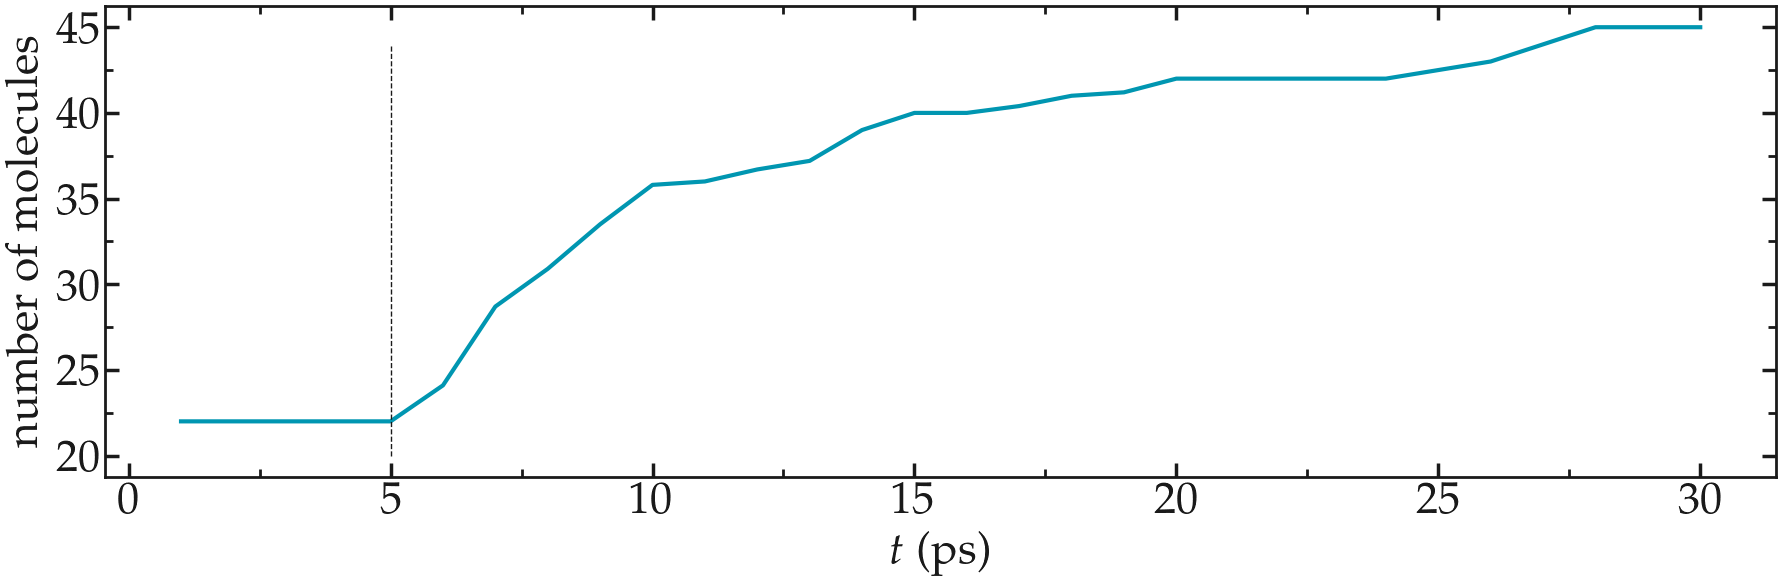
\includegraphics[width=\linewidth]{tutorials/level3/water-adsorption-in-silica/number_evolution-light.png}
\end{figure}

Note that the final number of molecules depends on the imposed pressure, 
temperature, and on the interaction between water and silica (its hydrophilicity). 

\hspace{-0.45cm}\begin{wrapfigure}{r}{4cm}
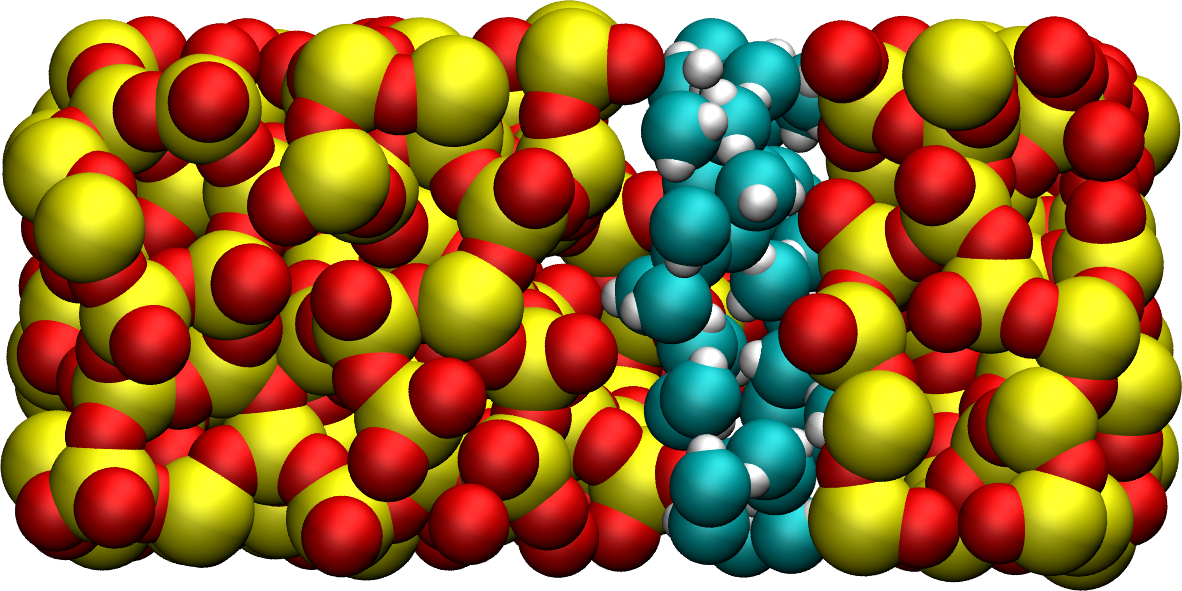
\includegraphics[width=4cm]{tutorials/level3/water-adsorption-in-silica/solvated-light.png}
\end{wrapfigure}

\noindent The figure on the side shows a snapshot of the final state, with the oxygen of the
water molecules represented in cyan.
Note that gcmc simulations of such dense phases are usually slow to converge due to the
very low probability of successfully inserting a molecule. Here, the short simulation 
duration was made possible by the use of a huge pressure.

\begin{tcolorbox}[colback=mylightblue!5!white,colframe=mylightblue!75!black,title=Vizualising varying number of molecules]
By default, VMD fails to properly render systems with varying number of atoms,
but Ovito does it well.
\end{tcolorbox}

\noindent \section{Exercises}

.. include:: ../../contact/requestsolution.rst

\subsection{Apply GCMC to water in ZIF-8 }

\noindent \hspace{-0.45cm}\begin{wrapfigure}{r}{4cm}
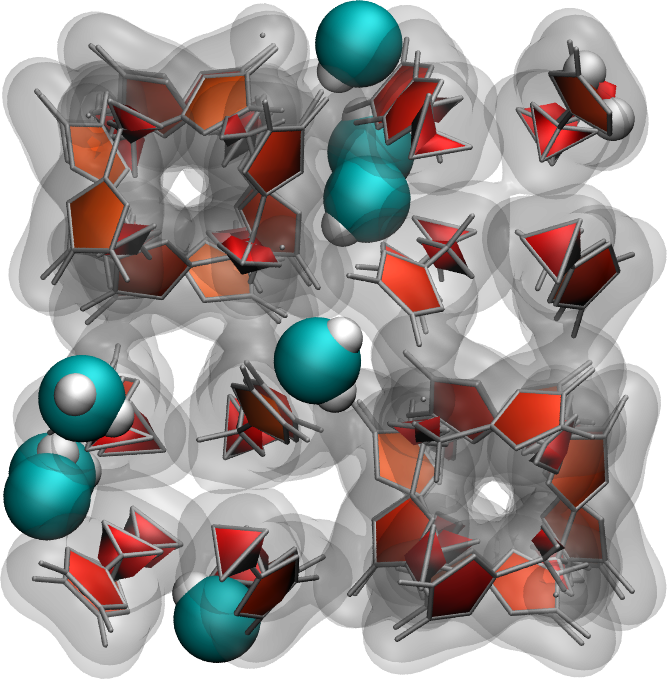
\includegraphics[width=4cm]{tutorials/level3/water-adsorption-in-silica/zif8-light.png}
\end{wrapfigure}

\noindent Use the same protocole as the one implemented in this tutorial to add water
molecules to a Zif-8 nanoporous material. A snapshot of the system with a 
few water molecules is presented on the right.
Download the initial Zif-8 \href{../../../../../inputs/level3/water-adsorption-in-silica/Exercises/Zif-8/zif-8.data}{structure}, the \href{../../../../../inputs/level3/water-adsorption-in-silica/Exercises/Zif-8/parm.lammps}{parameters} file, and this
new \href{../../../../../inputs/level3/water-adsorption-in-silica/Exercises/Zif-8/water.mol}{water template}. The ZIF-8 structure is made of 7 atom types (C1, C2, C3, H2, H3, N, Zn), connected
by bonds, angles, dihedrals, and impropers. It uses the same \textit{pair$\_$style} as water,
so there is no need to use the \textit{hybrid} functionality (see the hints below).
Note that, here, water occupies the atom types 1 and 2, instead of 3 and 4 in the case of SiO2.

\begin{tcolorbox}[colback=mylightblue!5!white,colframe=mylightblue!75!black,title=Hints]
Use the following parameters to start your LAMMPS input file.
\begin{lcverbatim}
units real
atom_style full
boundary p p p
bond_style harmonic
angle_style harmonic
dihedral_style hybrid charmm opls
improper_style harmonic
pair_style lj/cut/tip4p/long 1 2 1 1 0.105 14.0
kspace_style pppm/tip4p 1.0e-5
special_bonds lj 0.0 0.0 0.5 coul 0.0 0.0 0.833
\end{lcverbatim}

\noindent \end{tcolorbox}

